\chapter{Background}

\section{Wireless Communication}


\subsection{Problems with established wireless communication techniques}

\begin{figure}[h]
    \centering
    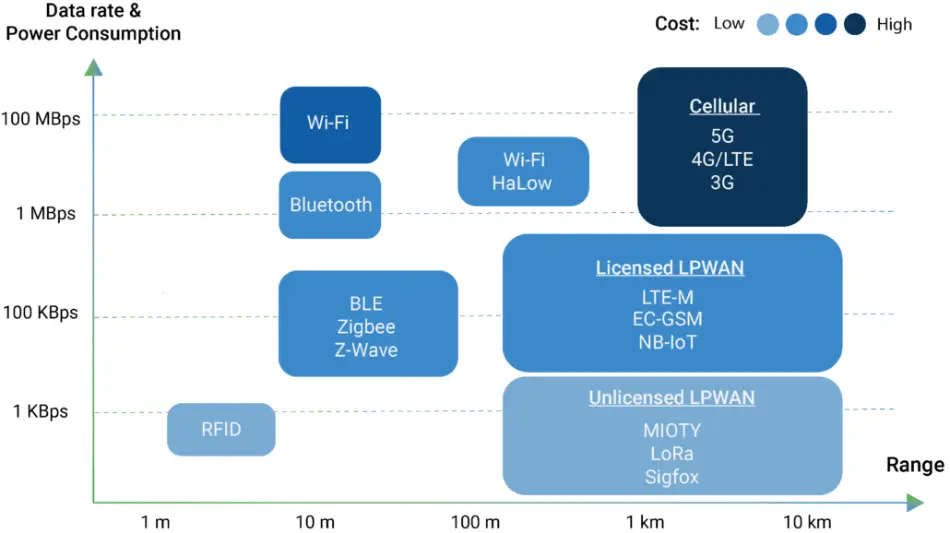
\includegraphics[width=1\textwidth]{pictures/lora/comparison-wireless-protocols.png}
    \caption{Comparison of data rate, power consumption and range between different wireless communication protocols~\protect\cite{wang_comparison_2021}}\label{pic:wireless-protocols-comparison}
\end{figure}

% show problems with current, widely used wireless communication techniques such as Wi-Fi, LTE, etc. 

While there are sensors that can be connected to the internet using Wi-Fi, ZigBee, \ac{LTE} and other, these technologies are not suitable for all use cases.

Deployments of sensors in remote areas, for example, might need long-range and low-power sensors that need to run on batteries for several years since replacing the batteries is expensive.
Likewise, sensors that are deployed in such areas can be hard to reach or placed apart by several hundred meters.

% TODO
Wi-Fi is not suitable for battery-powered devices that are deployed in remote areas, as it requires a lot of power to operate.
ZigBee is also not suitable for battery-powered devices, as it is not designed for long distances and thus has a very short range.
\ac{LTE} not suitable for battery-powered devices either as it requires a lot of power.
A rough comparison between selected wireless protocols can be seen in \cref{pic:wireless-protocols-comparison}~\cite{wang_comparison_2021}.

\subsection{\ac{RSSI} vs. \ac{SNR}}

\section{\acf{LoRa} modulation}

% explain the basics of LoRa with things like modulation, spreading factor, etc.
While, in the 868 MHz band used in the \ac{EU}, there are only a few channels available, \ac{LoRa} uses a technique called modulation to overcome this problem.


\subsection{Why use \ac{LoRa}?}

% todo: little power consumption, long range, low cost, etc. (link to diagram above)
As can be seen in \cref{pic:wireless-protocols-comparison}, \ac{LoRa} is a good choice for devices that need to be able to operate battery-powered in remote locations for extended periods of time, as it has a long range and low power consumption.

\subsection{Duty Cycle (in the \ac{EU} region)}

% TODO add a figure with the duty cycle

In the \ac{EU} region, the duty cycle for transmissions in the 868 MHz band is limited to 1\%~\cite{etsi_etsi_2012}.
This means that a \ac{LoRa} device using a frequency band in this range may only transmit for 1\% of a given time slot.
If, for example, a device transmits data for 36 seconds, it must stay silent for the following 3,564 seconds, which is almost an hour.
It needs to stay silent for the rest of the time.

Luckily, LoRa packets are usually only a few bytes small and can thus be transmitted in a short amount of time, usually in a few milliseconds.

\section{\acf{LoRaWAN}}

\begin{figure}[h]
    \centering
    
\includegraphics[width=.4\textwidth]{pictures/logos/LoRaWAN_Logo.eps}
    \caption{\ac{LoRaWAN} logo~\protect\cite{lora_alliance_francais_2022}}
\end{figure}

\ac{LoRaWAN} uses the LoRa wireless communication protocol to create a \ac{WAN} where multiple devices can communicate with each other over long distances.

\begin{figure}[h]
    \centering
    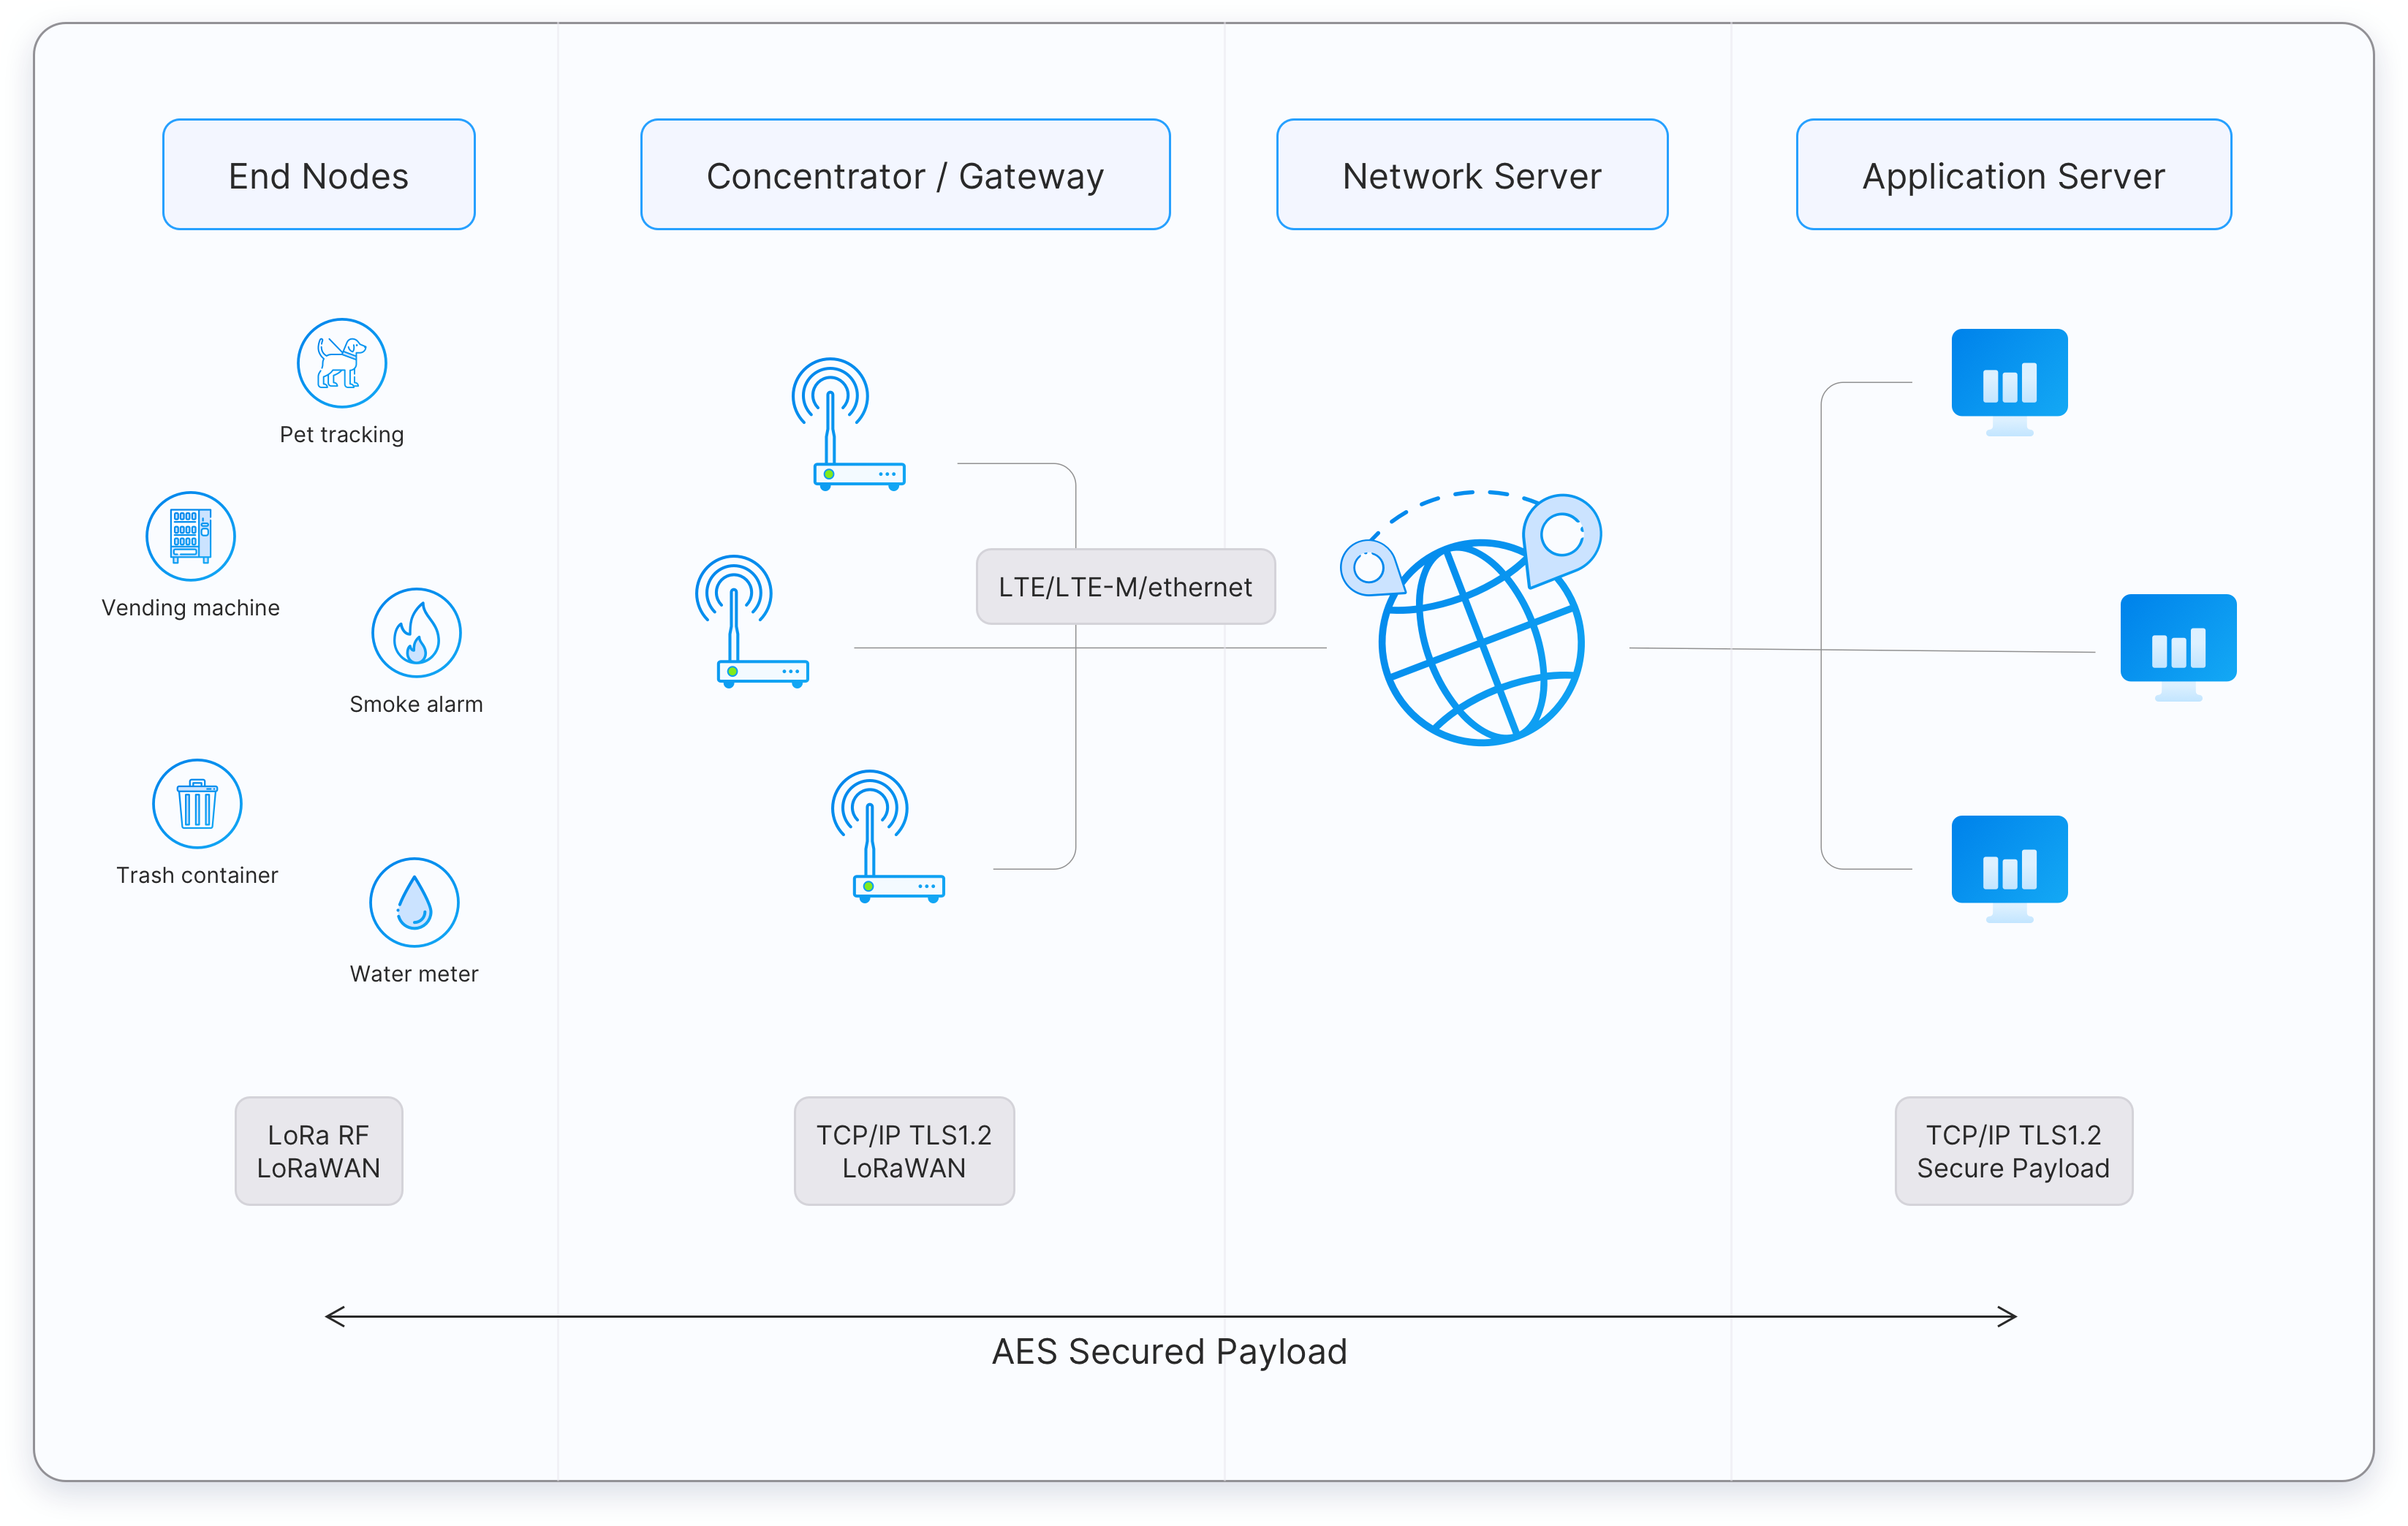
\includegraphics[width=1\textwidth]{pictures/lorawan-structure/lorawan-architecture.png}
    \caption{\ac{LoRaWAN} network structure~\protect\cite{the_things_industries_bv_lorawan_nodate}}\label{pic:lorawan-network-structure}
\end{figure}

The \ac{LoRaWAN} network architecture, as seen in \cref{pic:lorawan-network-structure} consists of four main components~\cite[p. 8]{lora_alliance_inc_lorawan_2017}:

\begin{itemize}
    \item the end nodes (also called devices or motes),
    \item the gateways (also called concentrators or base stations),
    \item the \ac{LNS}, and
    \item the \acp{AS}.
\end{itemize}

\ac{LoRaWAN} data rates typically range from 0.3 kbps to 50 kbps, depending on the region and the \ac{LoRa} modulation used~\cite[p. 8]{lora_alliance_inc_lorawan_2017}.

\subsection{Gateways}

\begin{figure}[h]
    \centering
    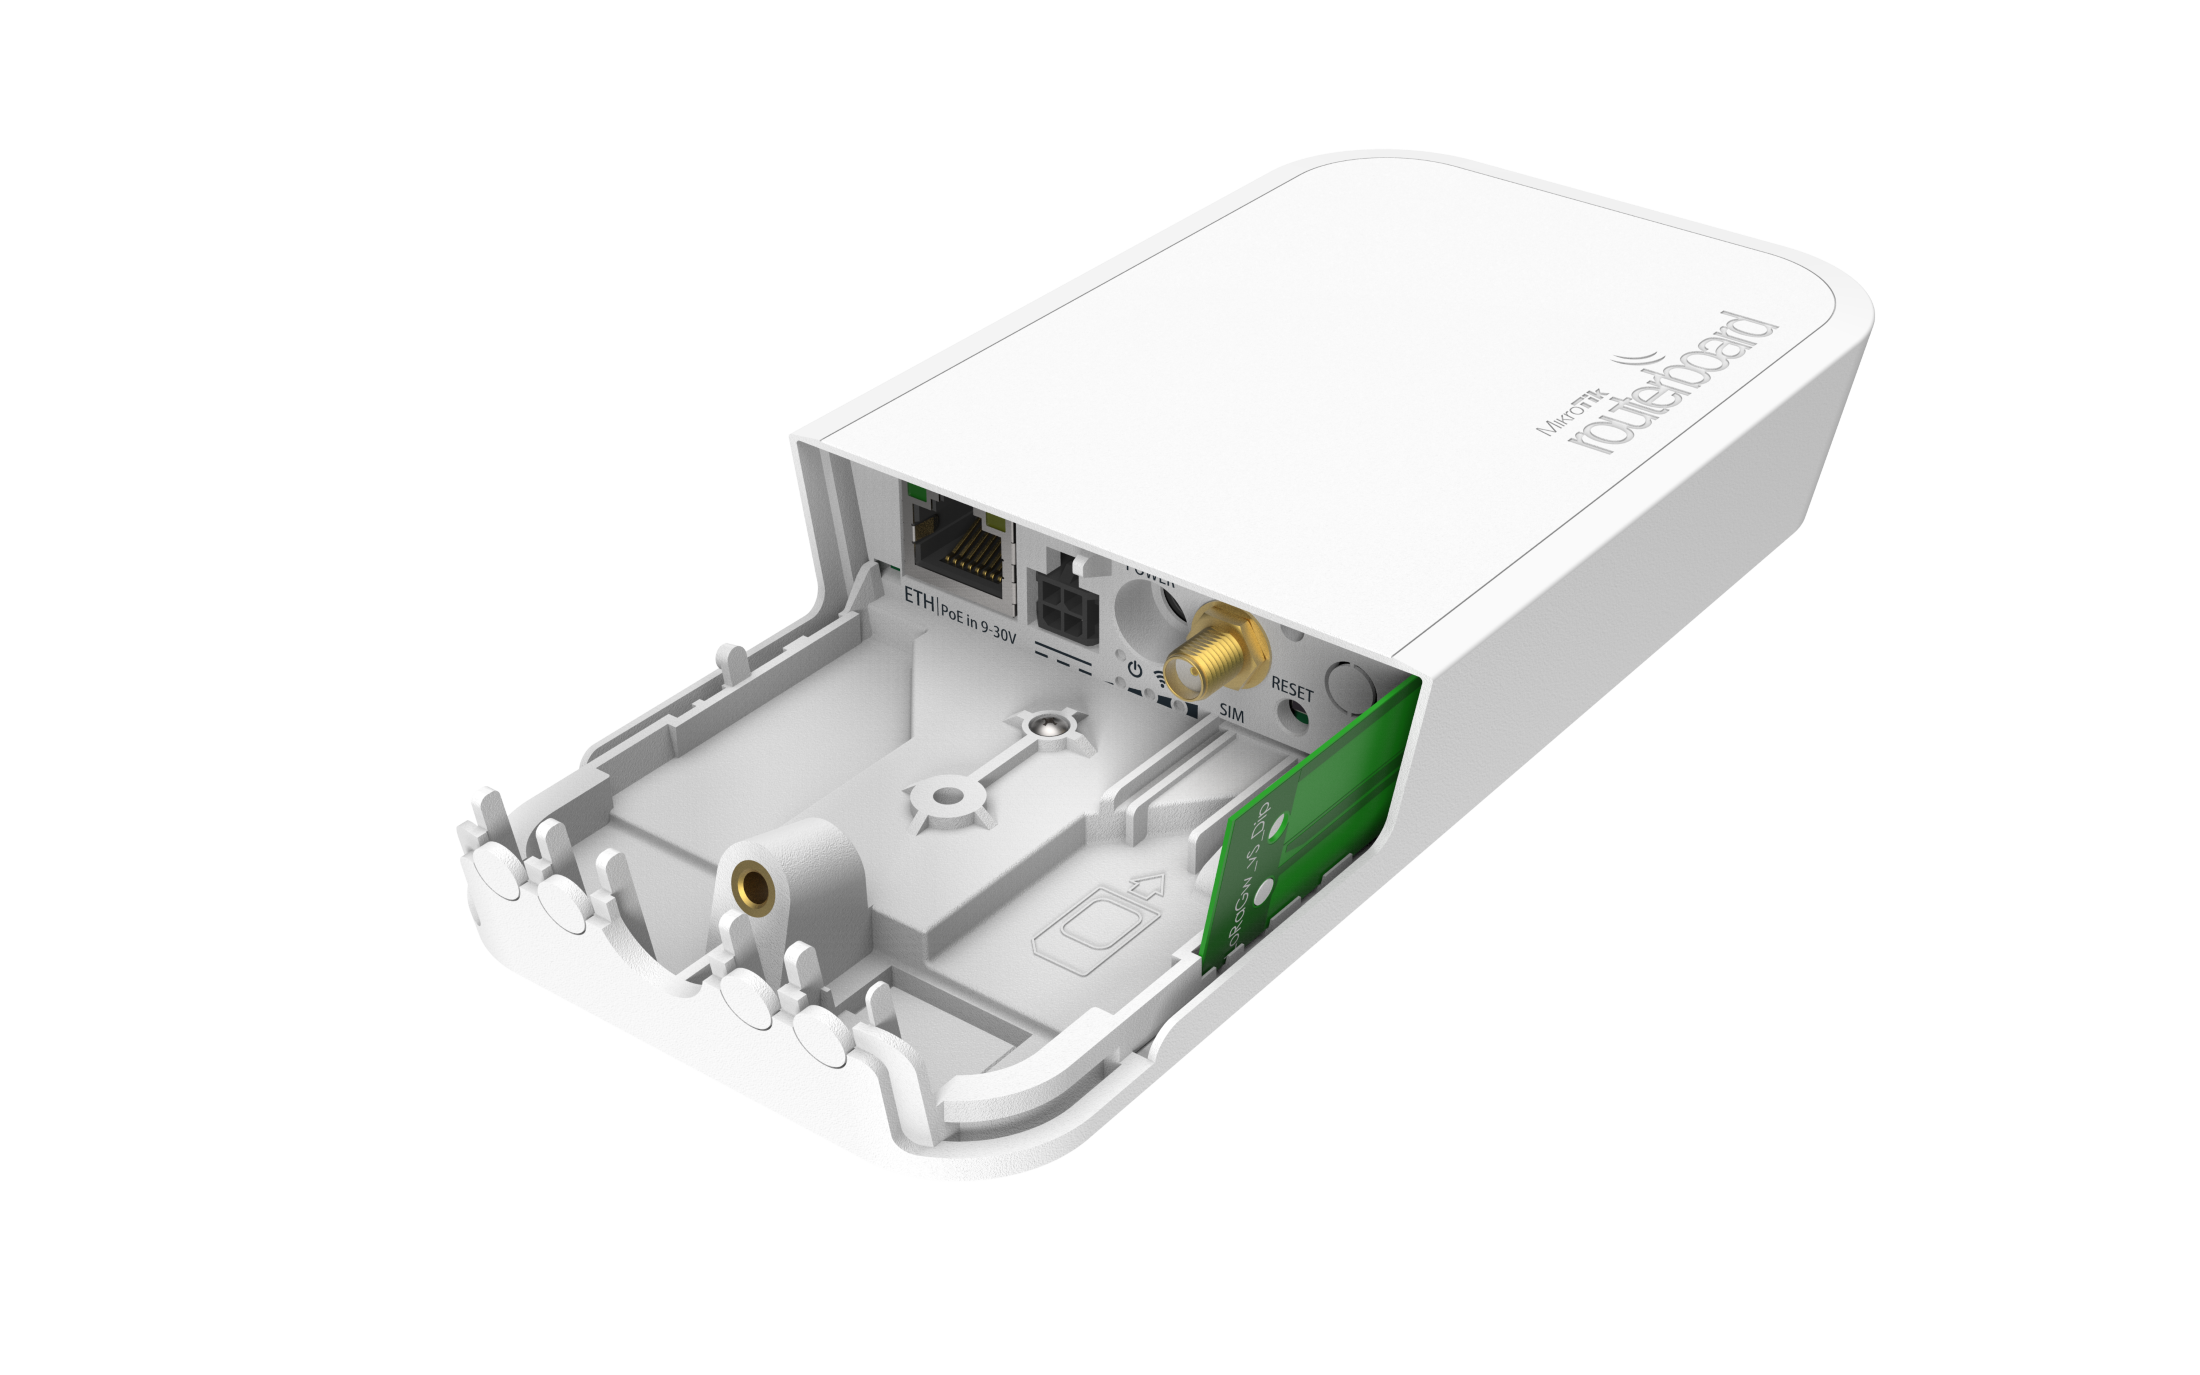
\includegraphics[width=.6\textwidth]{pictures/hardware/gateways/mikrotik-lr8-kit.png}
    \caption{MikroTik wAP LR8 kit Gateway~\protect\cite{the_things_industries_bv_lorawan_nodate}}\label{pic:mikrotik-lr8-kit-gateway}
\end{figure}

A \ac{LoRa} gateway is a device that receives \ac{LoRa} packets (usually from \ac{LoRa} nodes/end devices) and forwards them to the \ac{LoRaWAN} server.

\ac{LoRa} gateways are usually based on a \ac{LoRa} concentrator, which is a \ac{RF} front-end module that receives \ac{LoRa} packets and forwards them to the gateway's \ac{CPU} using a serial interface.
The \ac{CPU} processes the incoming data and forwards the packets to the \ac{LoRaWAN} server.

To achieve the connection to the \ac{LoRaWAN} server, the gateway needs to be connected to the internet.
This connection is a also called \emph{backhaul}.
The most widely used methods to realize this are Ethernet/\ac{LAN}, Wi-Fi and \ac{LTE} connections.

One example of a gateway used during this thesis and therein installed in Furtwangen is the \emph{MikroTik wAP LR8 kit}, as seen in \cref{pic:mikrotik-lr8-kit-gateway}.
This gateway is specified as suitable for outdoor usage, making it a good choice for the deployment in Furtwangen on top of (among others) the roof of the student dorm \ac{GHB}.

\begin{figure}[h]
    \centering
    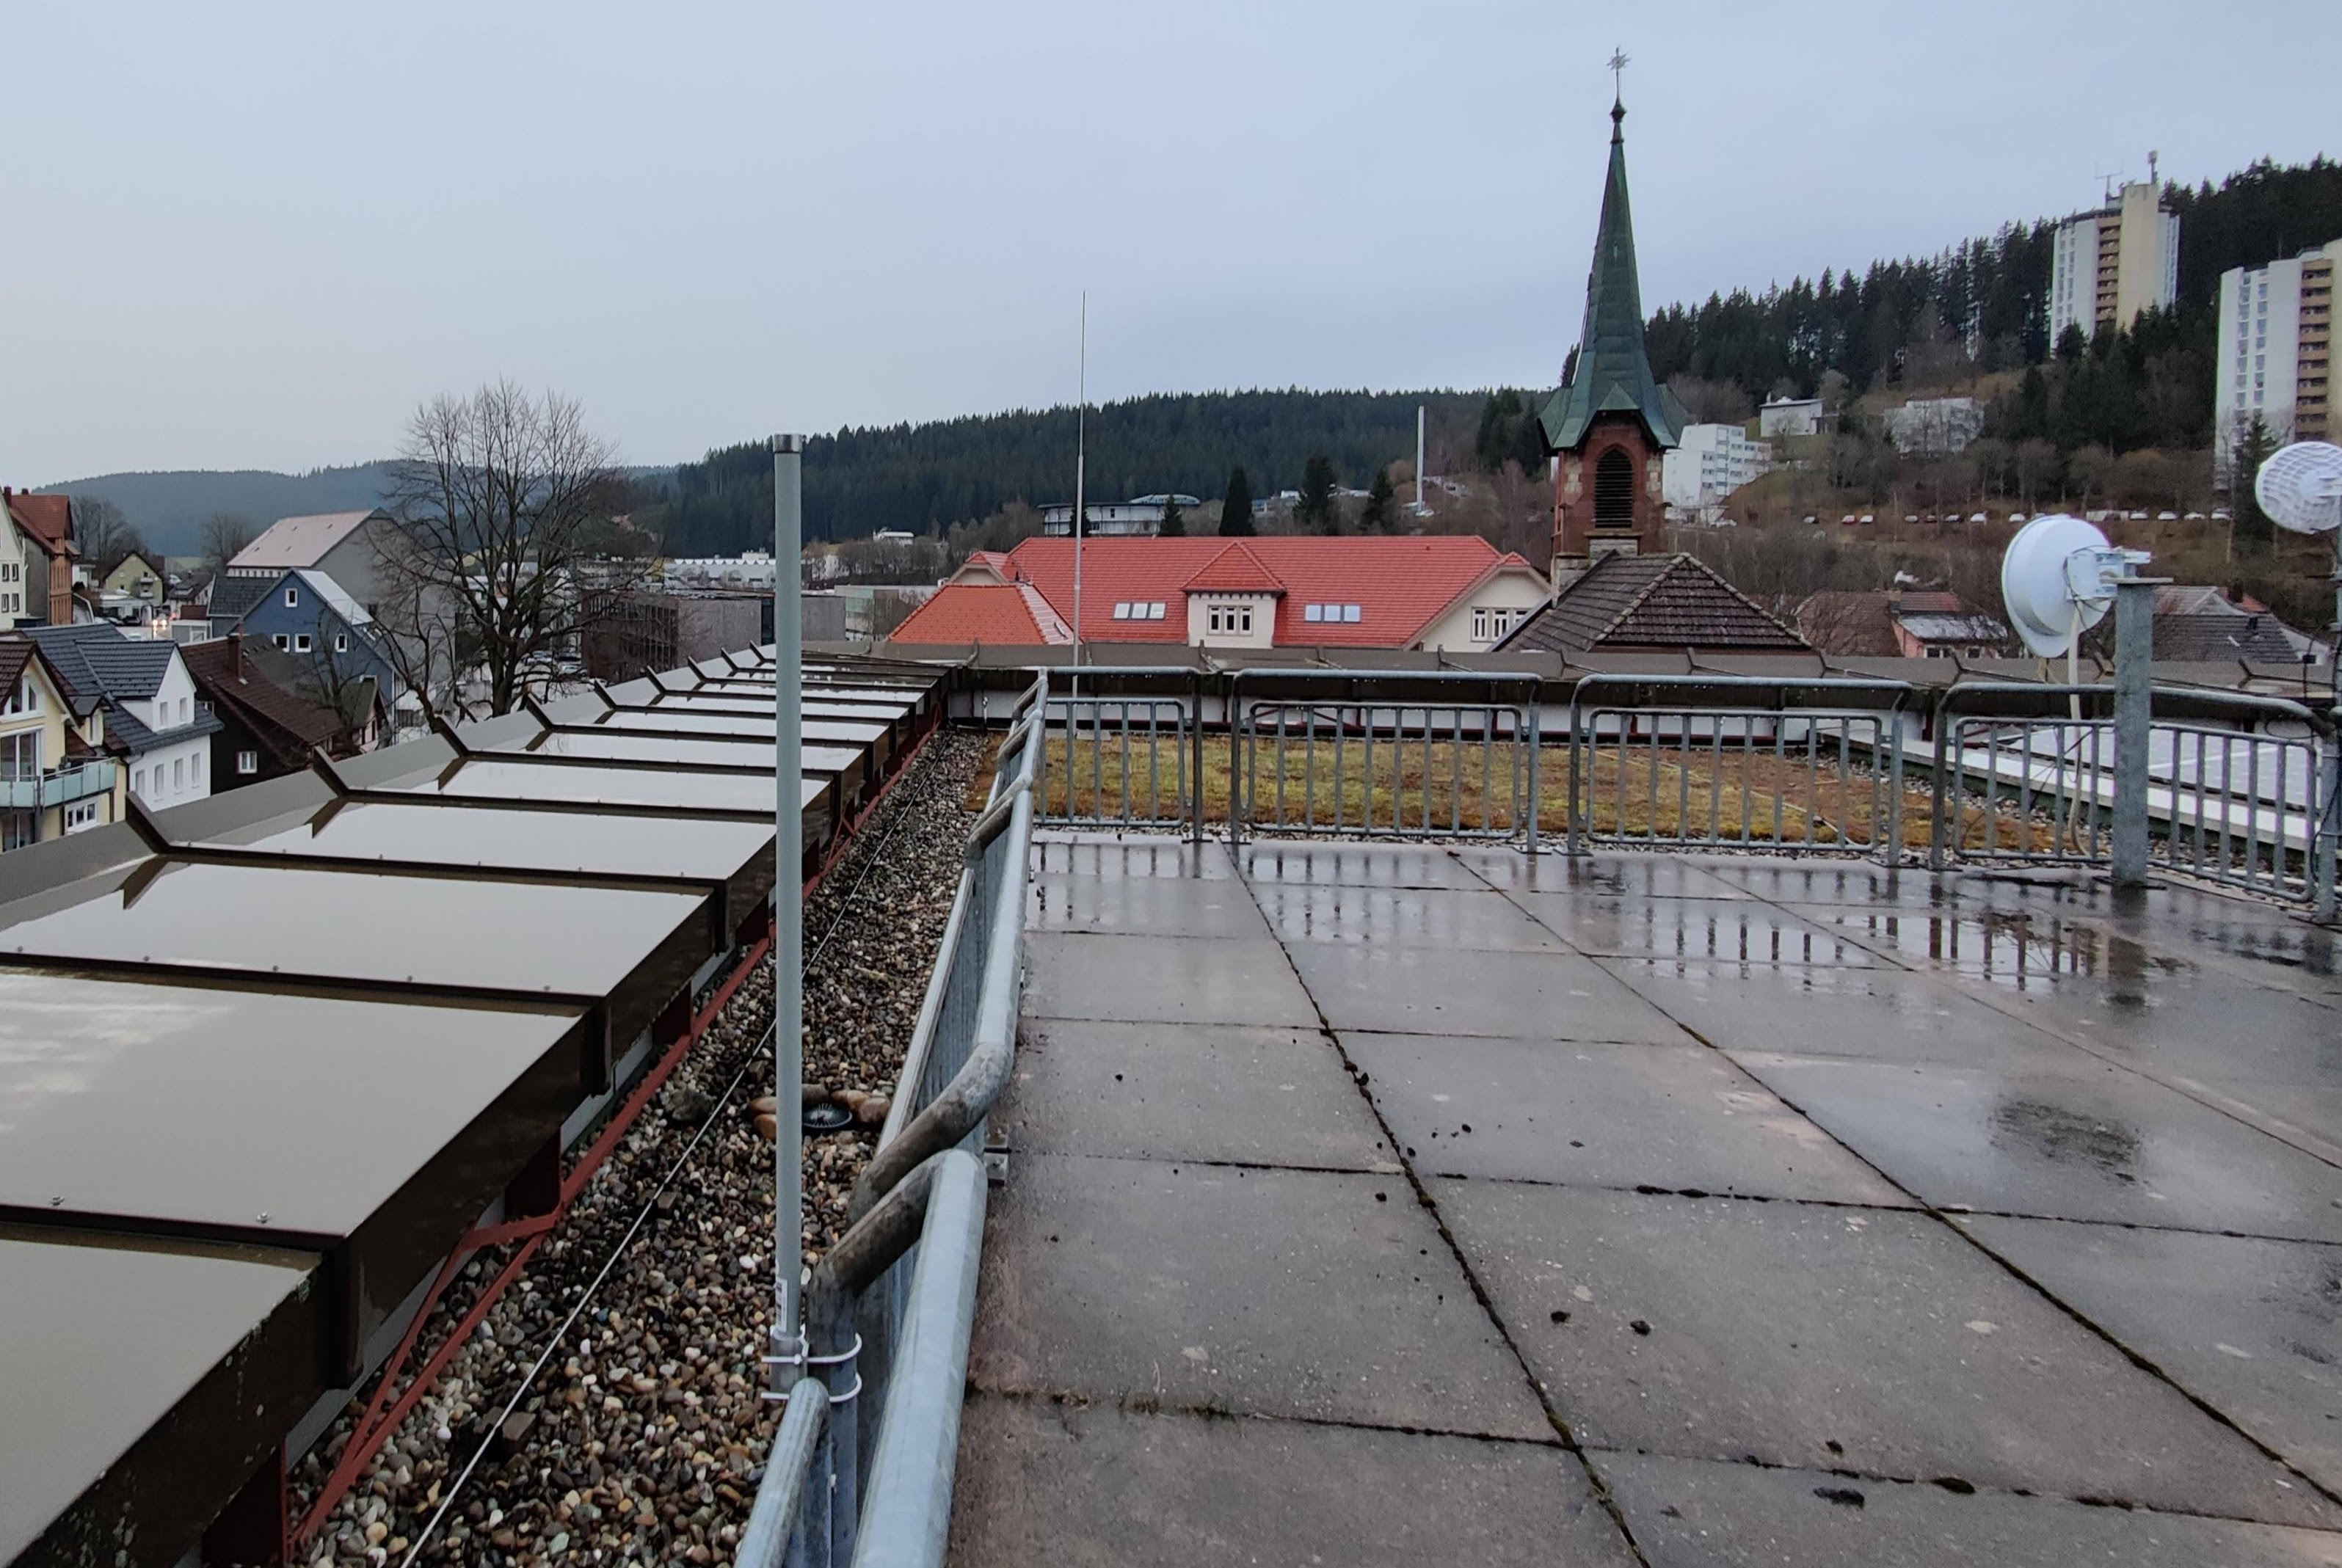
\includegraphics[width=0.6\textwidth]{pictures/hardware/gateway-deployment/mikrotik-antenna-c-building.jpg}
    \caption{The MikroTik antenna installed on top of the \ac{HFU} C building}\label{pic:mikrotik-antenna-c-building}
\end{figure}

While gateways like these usually have a built-in antenna, their range is only sufficient for covering small to medium-sized buildings or areas.
It is, however, also possible to use external antennas if it is necessary to cover a much larger area as was the case in this thesis since a medium to long range localization of \ac{LoRa} nodes was the goal.
While there are many choices for external antennas, as far as the MikroTik gateway is concerned, the choice was made to also use the external \ac{LoRa} antenna supplied by MikroTik, as it is specifically designed for the MikroTik gateway and thus should be a good match.
The deployment of this antenna on top of the \ac{HFU} C building is shown in \cref{pic:mikrotik-antenna-c-building}.

\subsection{Data Transmission}

In LoRaWAN, data transmissions to and from the end nodes are called \emph{uplink} and \emph{downlink}, respectively~\cite[p. 12]{lora_alliance_inc_lorawan_2017}.

Uplinks are relayed to the network server by one or more gateways from the end node.
Downlinks, however, are only sent from the network server to the end node using a single gateway.
\subsection{Device Classes}

\ac{LoRaWAN} defines three classes of devices that offer different variations of the trade-off between power consumption and data rate/availability~\cite[p. 10]{lora_alliance_inc_lorawan_2017}.

\subsubsection{Class A}

\begin{figure}[h]
    \centering
    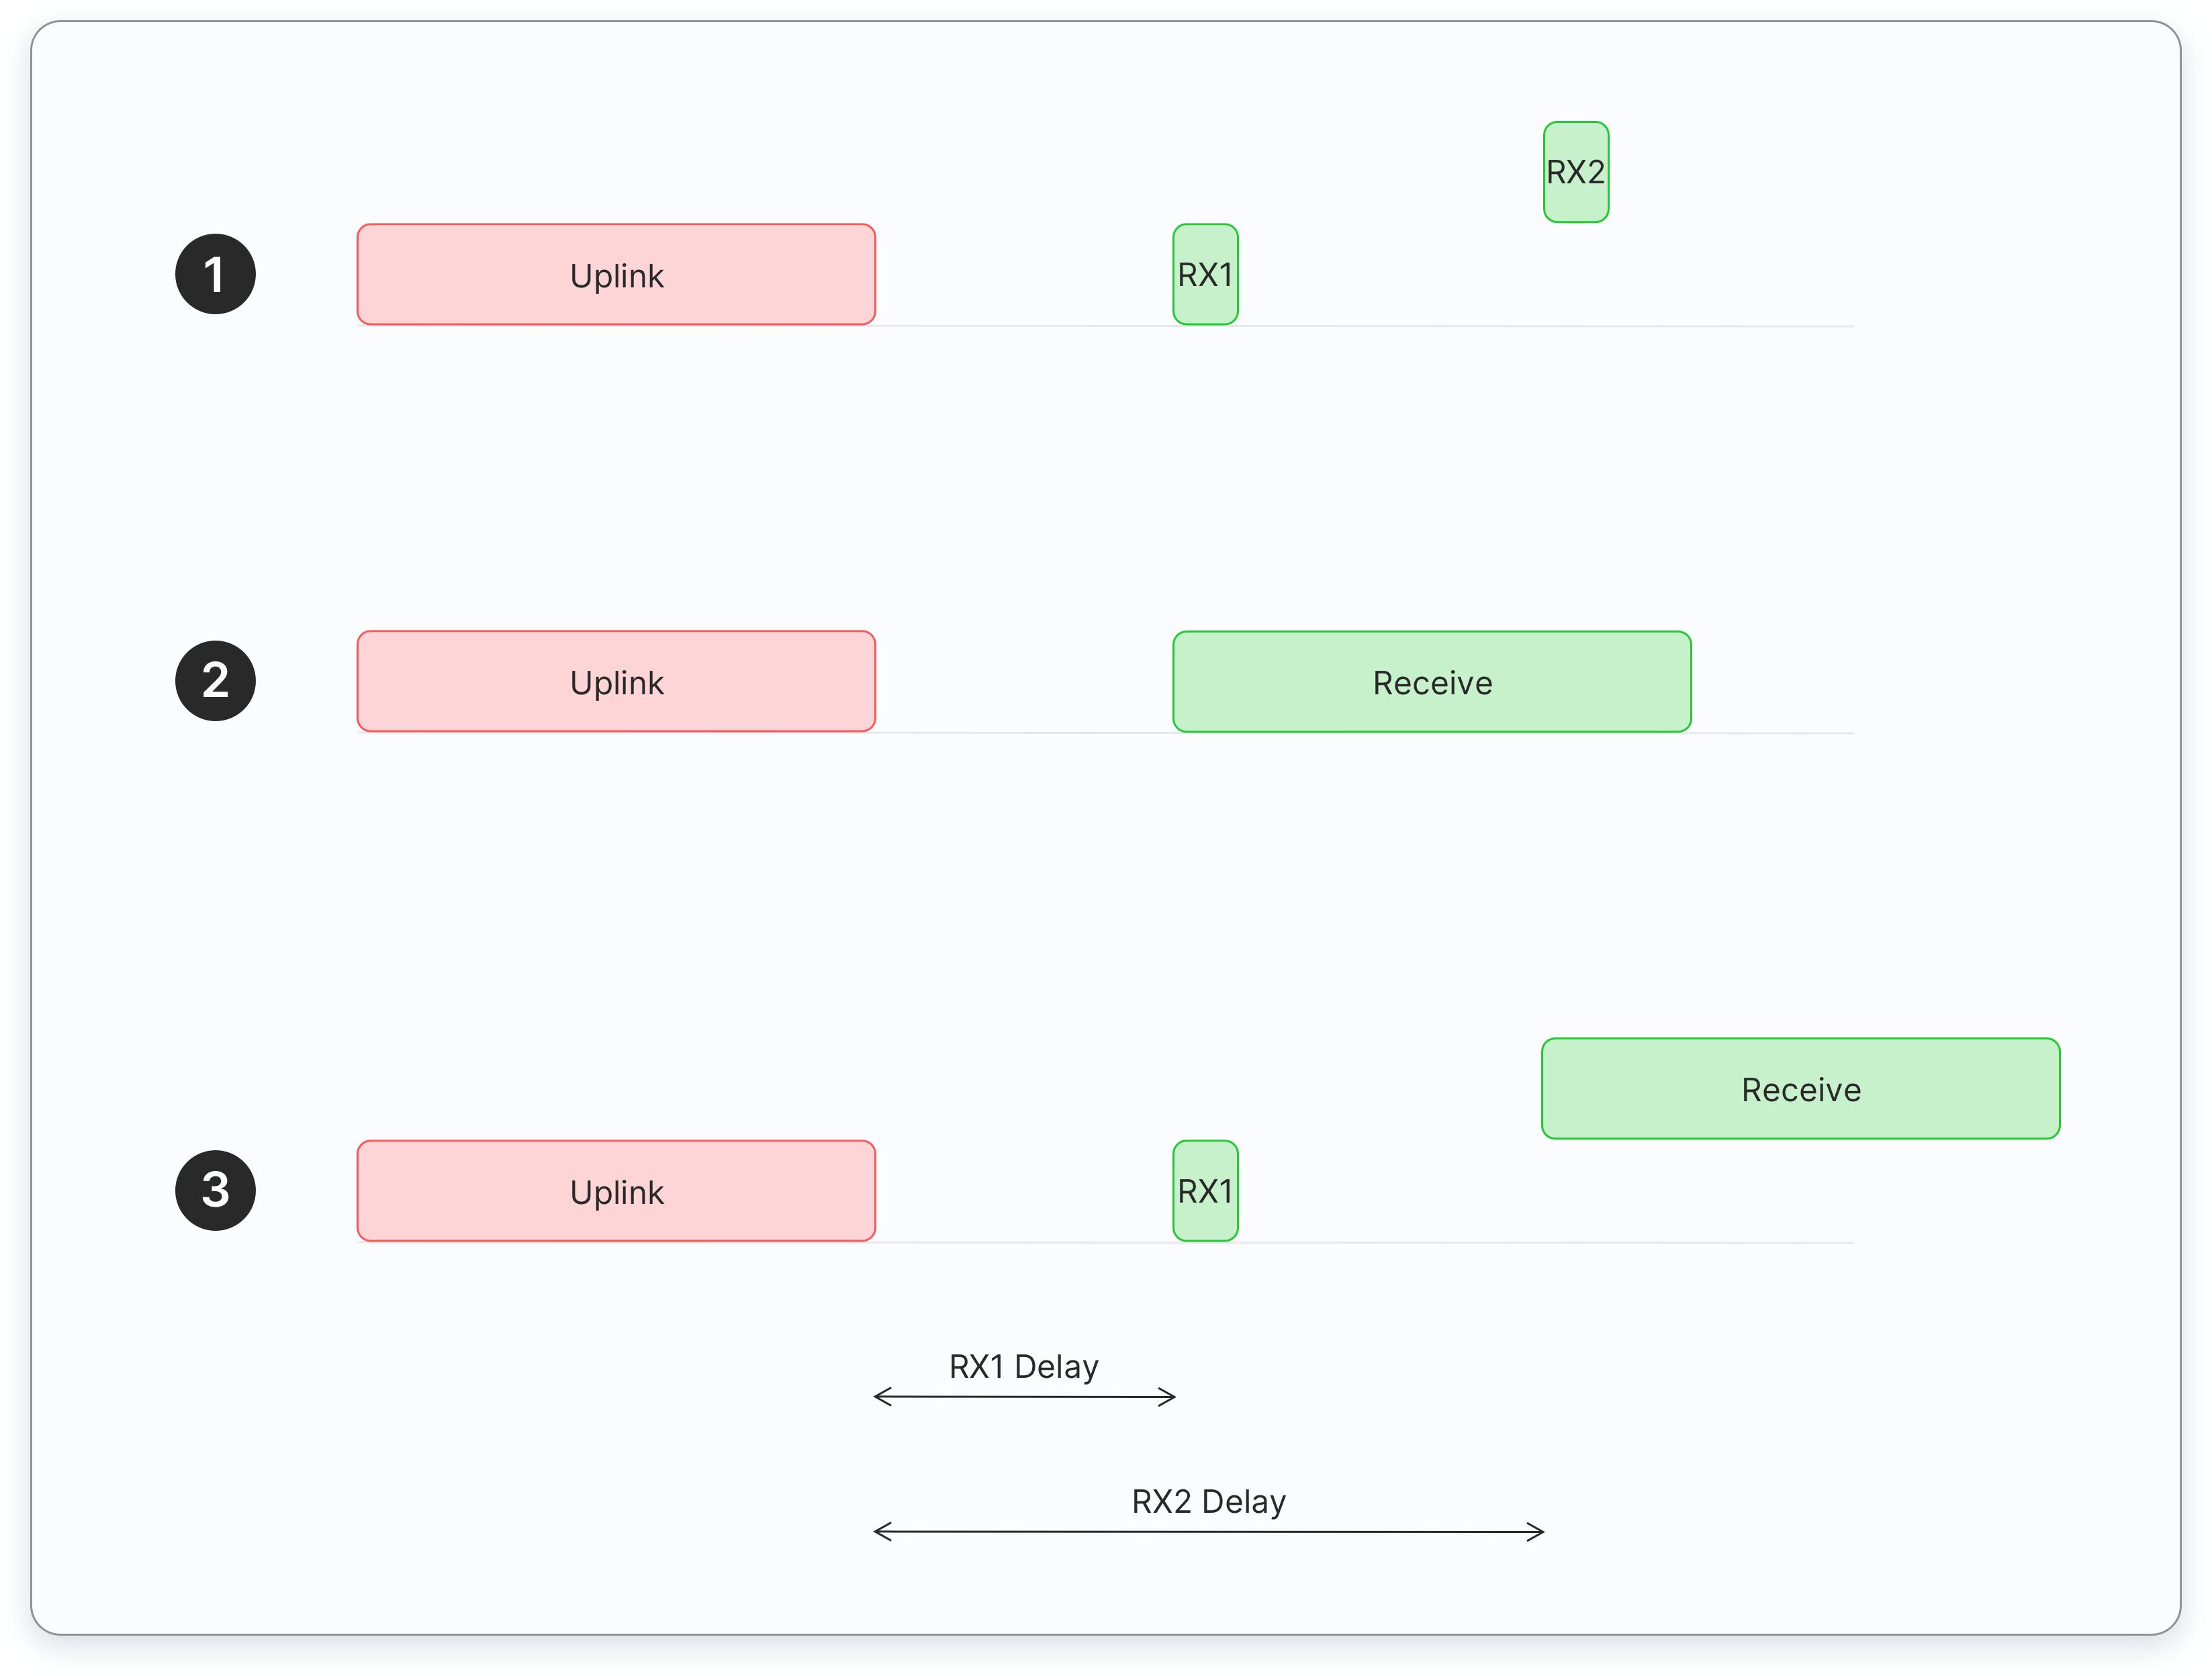
\includegraphics[width=1\textwidth]{pictures/device-classes/class-a.png}
    \caption{\ac{LoRaWAN} Device class A communication schema~\protect\cite{the_things_industries_bv_device_nodate}}\label{pic:lorawan-device-class-a-schema}
\end{figure}

Class A is used for devices that need to consume as little power as possible.
Every \ac{LoRaWAN} device must support the Class A mode~\cite[p. 11]{lora_alliance_inc_lorawan_2017}.
A communication in Class A is always initiated by the end device itself.

Bidirectional communication is possible in Class A through the use of two downlink receive windows during which it is possible for the \ac{LNS} to send data to the device.
This can be seen in \cref{pic:lorawan-device-class-a-schema}.
This also makes it impossible for the \ac{LNS} to send data to the device at any other time.

Class A consumes the least amount of power of the three classes, since the devices itself may specify when and how often they want to communicate with the \ac{LNS}.

\subsubsection{Class B}

\begin{figure}[h]
    \centering
    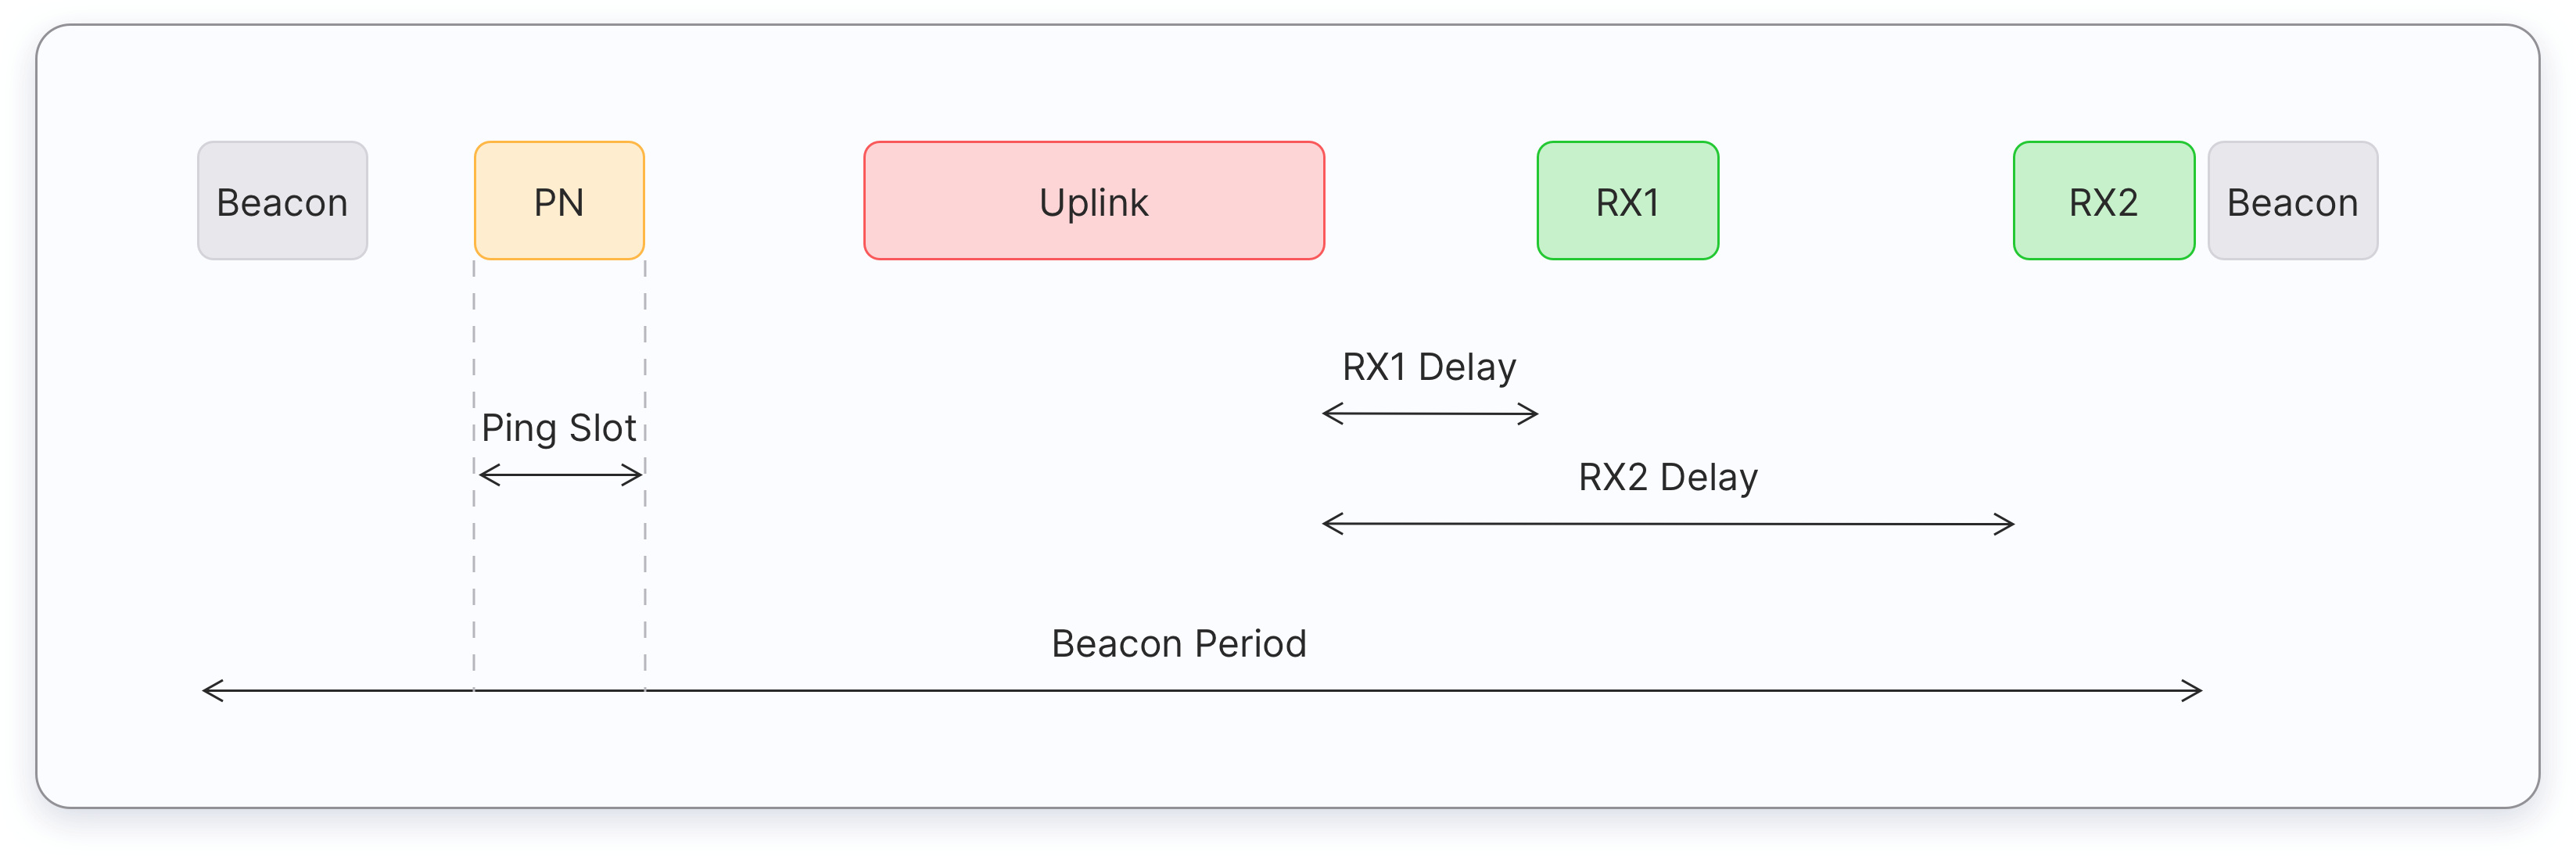
\includegraphics[width=1\textwidth]{pictures/device-classes/class-b.png}
    \caption{\ac{LoRaWAN} Device class B communication schema~\protect\cite{the_things_industries_bv_device_nodate}}\label{pic:lorawan-device-class-b-schema}
\end{figure}

In addition to class A, class B devices are also able to receive downlink messages from the \ac{LNS} during dedicated downlink receive windows.
In order to realize this without the need for a per-device \ac{RTC}, class B devices receive time synchronized beacons from the gateways.
The communication schema for class B devices can be seen in \cref{pic:lorawan-device-class-b-schema}.

These scheduled downlink windows result in a higher power consumption for class B devices, since those need to be awake during these windows.

\subsubsection{Class C}

\begin{figure}[h]
    \centering
    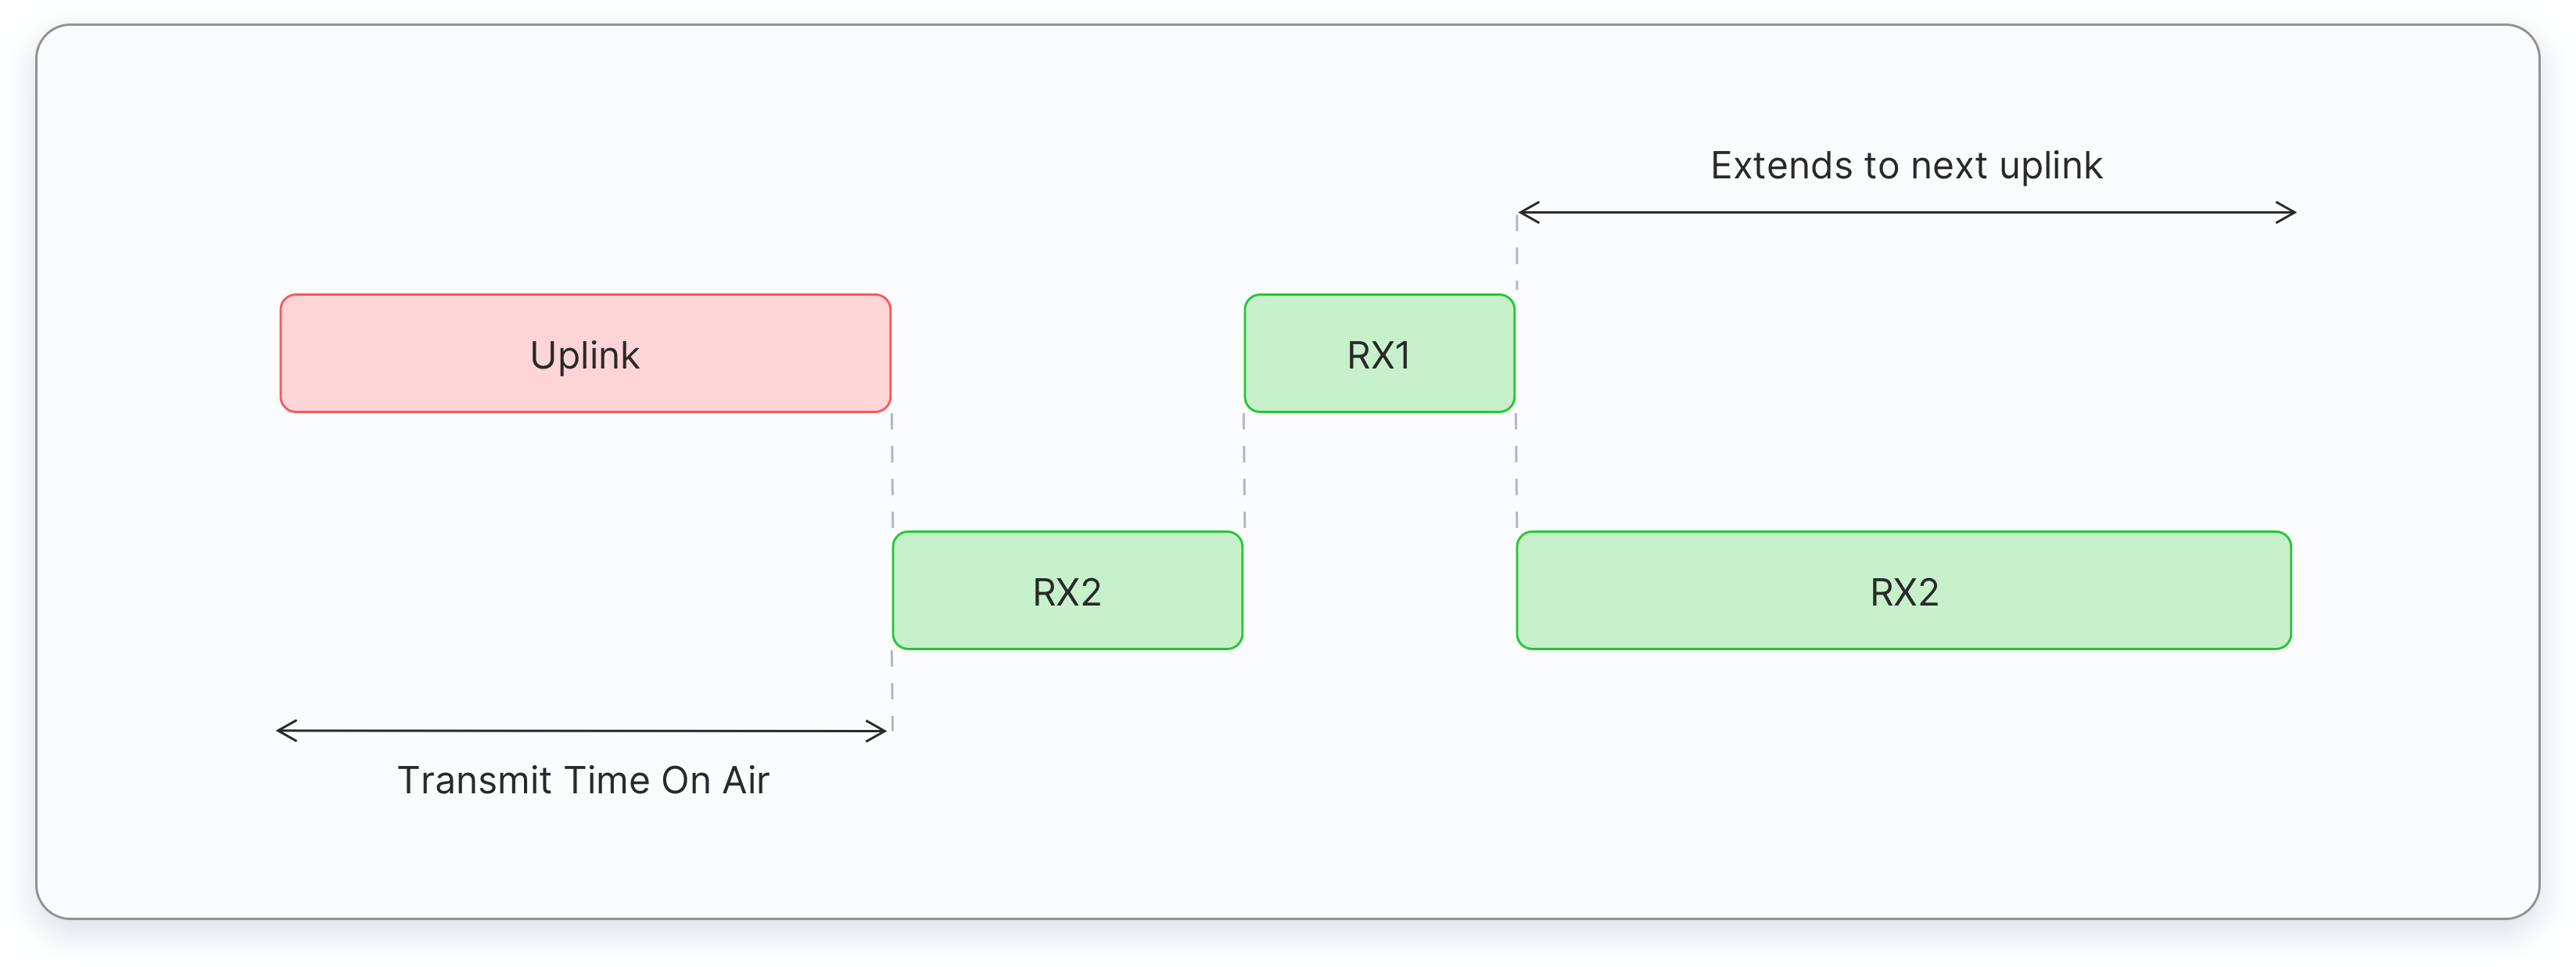
\includegraphics[width=1\textwidth]{pictures/device-classes/class-c.png}
    \caption{\ac{LoRaWAN} Device class C communication schema~\protect\cite{the_things_industries_bv_device_nodate}}\label{pic:lorawan-device-class-c-schema}
\end{figure}

Class C devices, when not currently transmitting an uplink message, are always listening for downlink messages from the \ac{LNS}.
In essence, they keep the downlink windows as specified in class B open all the time as seen in \cref{pic:lorawan-device-class-c-schema}.

Devices in class C consume the most power, since they are always listening for downlink messages.
The fact that they're always reachable by the \ac{LNS} also makes them the most suitable for applications that require a high data rate or a reliable accessibility via downlink.

\section{\acf{TTN}}

\begin{figure}[h]
    \centering
    
\includegraphics[width=0.3\textwidth]{pictures/logos/TTN-logo.eps}
    \caption{\acf{TTN} logo~\protect\cite{the_things_industries_bv_quick_nodate}}
\end{figure}

\ac{TTN} provides a free to use \ac{LNS} that supports a global community of people building \ac{LoRaWAN} applications.

While, officially, it is called \emph{The Things Stack Community Edition} since 2021, it is still commonly referred to as \acf{TTN}~\cite{the_things_industries_bv_what_2022}.
Its users provide \ac{TTN} with gateways that other users can use, making it a decentralized and crowdsourced \ac{LoRaWAN} network.

\subsection{Gateways}

Gateways can forward \ac{LoRaWAN} packets that it receives to the \ac{LNS} in two major ways:

\subsubsection{\acf{SUPF}}

The \acl{SUPF} is a piece of software used to connect \ac{LoRa} gateways to the \ac{LNS}~\cite{the_things_industries_bv_semtech_2022}.
The \ac{SUPF} relays \ac{LoRaWAN} packets that it receives from its connected \ac{LoRa} concentrator to the \ac{LNS} using the \ac{UDP} protocol.

It may be configured using JSON files such as \lstinline{global_conf.json} and \lstinline{local_conf.json}.

\ac{TTN} marked the \acl{SUPF} as deprecated, since it ``has many security and scalability drawbacks``~\cite{the_things_industries_bv_semtech_2022}.
It is advised to use the \acl{LBS} protocol instead.

\subsubsection{\acf{LBS}}

\begin{figure}[h]
    \centering
    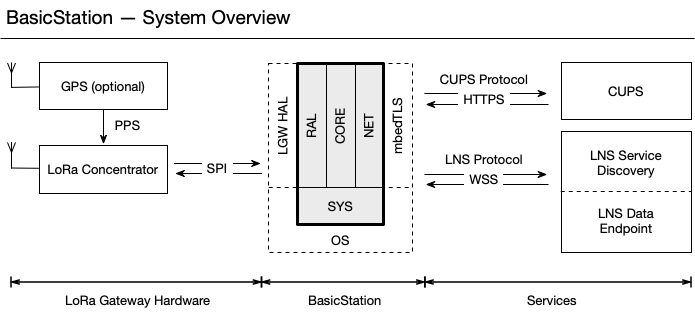
\includegraphics[width=0.9\textwidth]{pictures/lorawan-structure/lora-basics-station-structure.png}
    \caption{\acf{LBS} communication schema~\protect\cite{semtech_lora_developer_portal_lora_2022}}\label{pic:lora-basics-station-schema}
\end{figure}

Since \ac{TTN} v3, using the \ac{TCP}-based \acl{LBS} protocol is recommended over the \ac{SUPF} to connect gateways to the \ac{LNS}~\cite{the_things_industries_bv_semtech_2022}.

\ac{LBS} uses \ac{TLS}-encrypted \ac{TCP} connections with token-based authentication to relay \ac{LoRaWAN} packets to the \ac{LNS}~\cite{the_things_industries_bv_lora_2022}.

The two main components of \acl{LBS} are the \ac{LNS} itself as well as the \acf{CUPS}.
The communication schema can be seen in \cref{pic:lora-basics-station-schema}.

The \ac{LNS} is responsible for handling the \ac{LoRaWAN} packets whereas the \acl{CUPS} is responsible for handling the configuration of the gateways.

While \ac{CUPS} is not strictly necessary for sending actual \ac{LoRaWAN} packets, it simplifies the management of gateways and their configuration.
When a gateway is configured with \ac{CUPS}, it will automatically receive its configuration from the \ac{LNS} and be authenticated to work with it~\cite{the_things_industries_bv_lora_2022}.

\section{Localization of devices}

\subsection{Technologies}

This section will describe some technologies used in this thesis with the goal of making it easier to understand the topics being discussed.

\subsubsection{\ac{GPS}}

% Genauigkeit von GPS mit quelle
% GPS verwendet lateration -> quelle

\paragraph{\ac{HDOP}}

% Explain HDOP and relevance to GPS accuracy

\subsection{Triangulation}

\subsection{Multilateration}

\subsection{\acs{ToA}-based}

The \acf{ToA} based method uses the difference in the signal's time of arrival at the receiving stations.
In conjunction with the speed of light, this time difference can be used to calculate the distance between the receiving stations and the transmitting station.

\ac{ToA} is being used by radio location systems like \ac{GPS} to determine the position of a device by using Multilateration.

\subsection{\acs{TDoA}-based}

% how does it work

\subsection{\acs{RSSI}-based}

The method based on \acf{RSSI} uses the signal strength of the signal that is received.
Since signal strengths are not linear, the \ac{RSSI} values need to be converted to a linear scale.
Different devices can have different \ac{RSSI} values for the same distance.
\ac{RSSI} values can only function reliably when there is nothing blocking the signal between the transmitting and receiving stations, e.g. if there is a line of sight between the sender and receiver.

\section{\acf{TTNM}}

% What quotes to use?

\acf{TTNM} was created by JP Meijers in 2015. % Source: Linkedin profile okay?
While he first created it as a personal project to map the range of his own \ac{LoRaWAN} gateway, the project has since been expanded to map the coverages of almost all gateways registered in the public \ac{TTN} network.

% explain how it works in conjunction with TTN

\acl{TTNM} works by using \ac{LoRaWAN} nodes with \ac{GPS} modules that send their location to the \ac{TTN} network via uplink messages.
Alongside the location information, those nodes' messages also include information about which gateways received the message.
Hence, \acl{TTNM} can use the information about which gateways received the message and the location information of the nodes' \ac{GPS} modules to build a map displaying the coverage of \ac{LoRaWAN} gateways in the \ac{TTN} network.

% explain why it is important for the thesis

As far as this thesis is concerned, \acl{TTNM} is important because it provided a way to access \ac{RSSI} and location data points for measurements done by \ac{GPS}-enabled \ac{LoRaWAN} nodes.